\section{Анализ предметной области}
\subsection{История развития веб-мессенджеров}

История веб-мессенджеров тесно связана с развитием интернет-технологий и появлением средств онлайн-коммуникации. Этот жанр программного обеспечения стал неотъемлемой частью современного общения в виртуальном пространстве. Вот краткая история развития веб-мессенджеров:

\begin{enumerate}
	\item \textbf{IRC и ICQ (1990-е годы):} Первыми формами онлайн-чата были интернет-ретрансляции (IRC), позволяющие пользователям общаться в реальном времени. В середине 1990-х годов появилась ICQ, первая широко распространенная программа мгновенного обмена сообщениями, что сделало общение в сети более доступным.
	
	\item \textbf{AIM, MSN Messenger, Yahoo Messenger (2000-е годы):} В 2000-х годах появились AIM (AOL Instant Messenger), MSN Messenger и Yahoo Messenger. Они предложили дополнительные функции, такие как передача файлов, видеозвонки и персонализированные статусы.
	
	\item \textbf{Skype и Google Talk (2000-е годы):} Skype и Google Talk (позднее ставший частью Google Hangouts) предоставили пользователям возможность совершения голосовых и видеозвонков, расширяя возможности коммуникации.
	
	\item \textbf{WhatsApp, Telegram, и Viber (2010-е годы):} С массовым распространением смартфонов в 2010-х годах, приложения мессенджеров на основе мобильных платформ, такие как WhatsApp, Telegram и Viber, стали популярными, предлагая шифрование сообщений и другие расширенные функции.
	
	\item \textbf{Современные веб-мессенджеры (2020-е годы):} С появлением современных веб-мессенджеров, таких как Slack, Microsoft Teams, и Discord, область коммуникаций в корпоративном и геймерском сегментах значительно разнообразилась. Эти приложения интегрируют функциональности чата с коллективной работой, обменом файлами и другими возможностями.
	
\end{enumerate}

История веб-мессенджеров демонстрирует постоянное развитие средств онлайн-коммуникации, от простых текстовых чатов до многофункциональных приложений, объединяющих в себе различные аспекты виртуального общения.

\subsection{Веб-мессенджер: особенности и тенденции}
Веб-мессенджер – это приложение, предназначенное для обмена мгновенными сообщениями в режиме реального времени через сеть интернет. Основные особенности и тенденции веб-мессенджеров включают:

\begin{enumerate}
	\item \textbf{Многоплатформенность:} Современные веб-мессенджеры обеспечивают поддержку различных платформ, включая веб-версии, мобильные приложения и настольные приложения.
	
	\item \textbf{Безопасность и шифрование:} В ответ на повышенный интерес к безопасности в сети, веб-мессенджеры внедряют технологии шифрования сообщений для защиты конфиденциальности пользователей.
	
	\item \textbf{Интеграция с другими сервисами:} Современные мессенджеры предоставляют интеграцию с другими сервисами и приложениями, такими как облачные хранилища, календари, видеоконференции, что обогащает опыт пользователей.
	
	\item \textbf{Коллективная работа:} Веб-мессенджеры для бизнеса (например, Slack, Microsoft Teams) акцентируют внимание на коллективной работе, предоставляя инструменты для обмена файлами, обсуждения проектов и интеграции с рабочими инструментами.
	
	\item \textbf{Использование искусственного интеллекта:} Некоторые веб-мессенджеры начинают использовать искусственный интеллект для улучшения опыта пользователей, предоставляя персонализированные рекомендации и автоматизированные задачи.
	
\end{enumerate}

Тенденции веб-мессенджеров продолжают эволюцию в ответ на изменяющиеся потребности пользователей и бизнеса, что подчеркивает их важность в современной коммуникационной экосистеме.

\begin{figure}
	\centering
	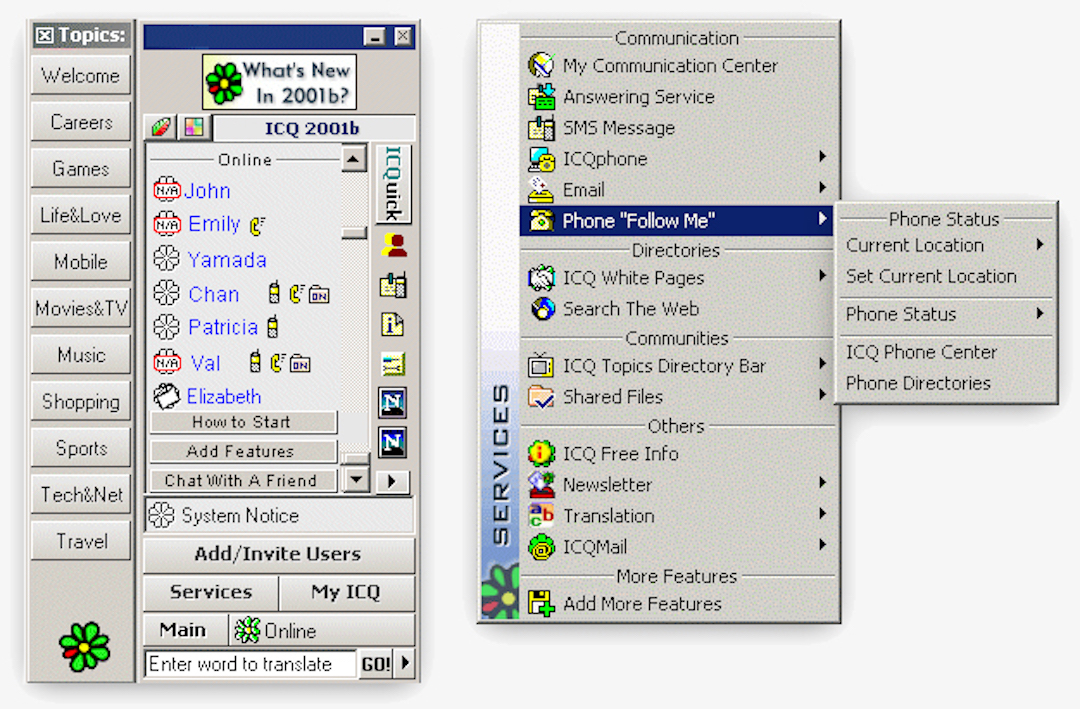
\includegraphics[width=0.7\linewidth]{images/icq}
	\caption{Первый мессенджер ICQ}
	\label{fig:icq}
\end{figure}

\begin{figure}
	\centering
	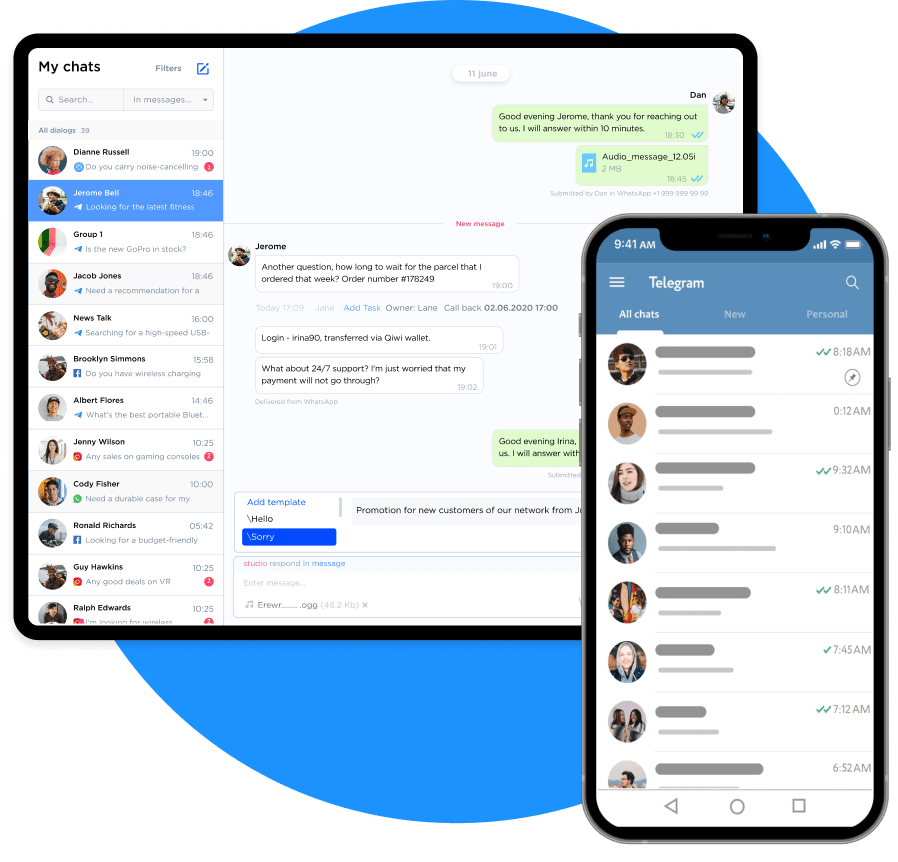
\includegraphics[width=0.7\linewidth]{images/telegram}
	\caption{Популярный мессенджер Telegram}
	\label{fig:telegram}
\end{figure}
